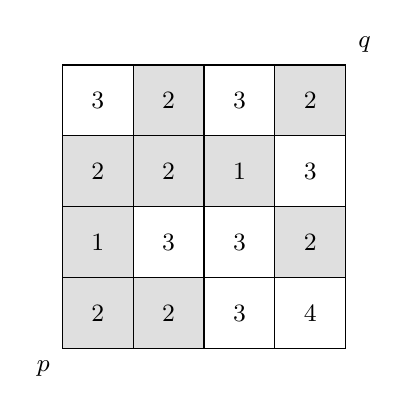
\begin{tikzpicture}[scale=0.9, every node/.style={font=\small}][H]
  %----- 基本參數 -----
  \def\cell#1#2#3{ % (row, col, value)
    % 座標:左下(1,1),右上(4,4);但我們用 top-down 排列所以要轉換
    \pgfmathsetmacro{\x}{#2-1}
    \pgfmathsetmacro{\y}{4-#1}
    % 填色:V={1,2} 可走(light gray),其他白色
    \ifnum#3<3
      \fill[gray!25] (\x,\y) rectangle ++(1,1);
    \else
      \fill[white]   (\x,\y) rectangle ++(1,1);
    \fi
    % 外框
    \draw (\x,\y) rectangle ++(1,1);
    % 數字
    \node at (\x+0.5,\y+0.5) {\small #3};
  }
  %----- 填資料(row, col, value) -----
  % Row 1 (top): 3 2 3 2(q)
  \cell{1}{1}{3}  \cell{1}{2}{2}  \cell{1}{3}{3}  \cell{1}{4}{2}
  % Row 2: 2 2 1 3
  \cell{2}{1}{2}  \cell{2}{2}{2}  \cell{2}{3}{1}  \cell{2}{4}{3}
  % Row 3: 1 3 3 2
  \cell{3}{1}{1}  \cell{3}{2}{3}  \cell{3}{3}{3}  \cell{3}{4}{2}
  % Row 4 (bottom): 2(p) 2 3 4
  \cell{4}{1}{2}  \cell{4}{2}{2}  \cell{4}{3}{3}  \cell{4}{4}{4}

  %----- 標記 p 與 q -----
  % p at (row=4,col=1) -> (x=0,y=0)
  \node[below left=1pt] at (0,0) {$p$};
  % q at (row=1,col=4) -> (x=3,y=3)
  \node[above right=1pt] at (4,4) {$q$};

%   %----- shortest-8(藍色,長度 4): p(4,1)->(3,1)->(2,2)->(2,3)->q(1,4) -----
%   \draw[very thick,blue,-{Stealth[length=3mm]}]
%     (0.5,0.5) -- (0.5,1.5) -- (1.5,2.5) -- (2.5,2.5) -- (3.5,3.5);

%   %----- shortest-m(橙色,長度 5): p->(3,1)->(2,1)->(2,2)->(2,3)->q -----
%   \draw[very thick,orange!90!black,-{Stealth[length=3mm]}]
%     (0.5,0.5) -- (0.5,1.5) -- (0.5,2.5) -- (1.5,2.5) -- (2.5,2.5) -- (3.5,3.5);

%   %----- 圖例 -----
%   \draw[very thick,blue]   (0.1,-0.7)--+(0.6,0) node[right,black]{shortest-8 length $=4$};
%   \draw[very thick,orange!90!black] (2.6,-0.7)--+(0.6,0) node[right,black]{shortest-m length $=5$};
%   \node[black] at (2,-1.2) {shortest-4: no 4-connected path (q is 4-blocked)};
\end{tikzpicture}